\documentclass[text01.tex]{subfiles}
\begin{document}
%
% section 1.5
%
\section{\ruby{電源}{でんげん}の切り方を覚えよう}

\ruby{皆}{みな}さんのデータもそうですが、ラズベリーパイのすべてのデータは、microSDカードに\ruby{保存}{ほぞん}されています。
そのため、いきなり\ruby{電源}{でんげん}を切ってしまうと、microSDカードに書き\ruby{込}{こ}んでる途中や書き\ruby{込}{こ}まれる前に
\ruby{電源}{でんげん}が切れてしまい、データが\ruby{壊}{こわ}れてしまう\ruby{可能性}{かのうせい}があります。

\ruby{電源}{でんげん}を切る\ruby{際}{さい}は、決められた手順に\ruby{従}{したが}う必要があります。
ラズベリーパイを使い終わったら正しい手順で\ruby{電源}{でんげん}が切れるように覚えておきましょう。
\bigskip

{\bf \ruby{電源}{でんげん}を切る手順}

\noindent%
  \begin{minipage}[t]{0.44\columnwidth}
    \textcircled{\scriptsize{1}}\\
    ラズベリーのアイコンをクリックしてメニューを開きます。一番下の「ログアウト」をクリックしてください。
  \end{minipage}\hfill
  %
  \begin{minipage}[t]{0.55\columnwidth}
    \centering
    \vbox to 0pt{\vskip-3mm
      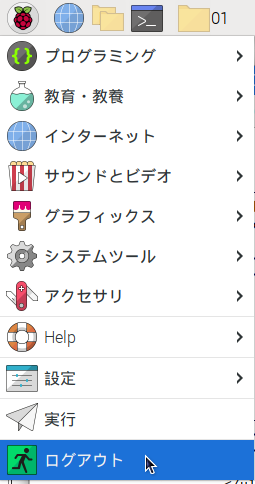
\includegraphics[keepaspectratio, height=55mm]{../../asset/image/textbook-img206.png}
    \vss}
    \vspace{60mm}
  \end{minipage}
%
\begin{minipage}[t]{0.44\columnwidth}
  \textcircled{\scriptsize{2}}\\
  右の図のようなウィンドウが表示されます。
  一番上の「Shutdown」ボタンをクリックして\ruby{電源}{でんげん}を切りましょう。
\end{minipage}\hfill
%
\begin{minipage}[t]{0.55\columnwidth}
  \centering
  \vbox to 0pt{\vskip-3mm
    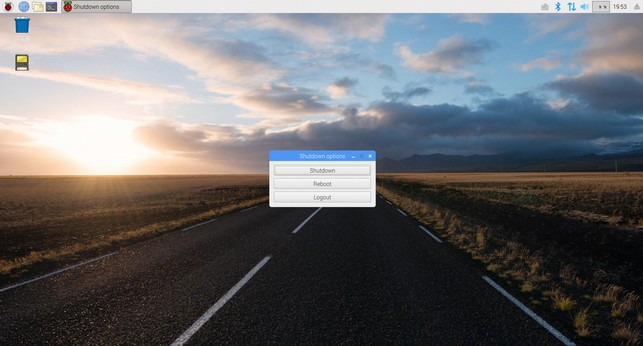
\includegraphics[keepaspectratio, height=40mm]{../../asset/image/textbook-img208.jpg}
  \vss}
  \vspace{45mm}
\end{minipage}
%
\begin{minipage}[t]{0.44\columnwidth}
  \textcircled{\scriptsize{3}}\\
  ラズベリーパイ本体の緑色のランプが\ruby{消灯}{しょうとう}します。
  この\ruby{状態}{じょうたい}が確認できたら、アダプターをコンセントから抜きましょう。
\end{minipage}\hfill
%
\begin{minipage}[t]{0.55\columnwidth}
  \centering
  \vbox to 0pt{\vskip-3mm
    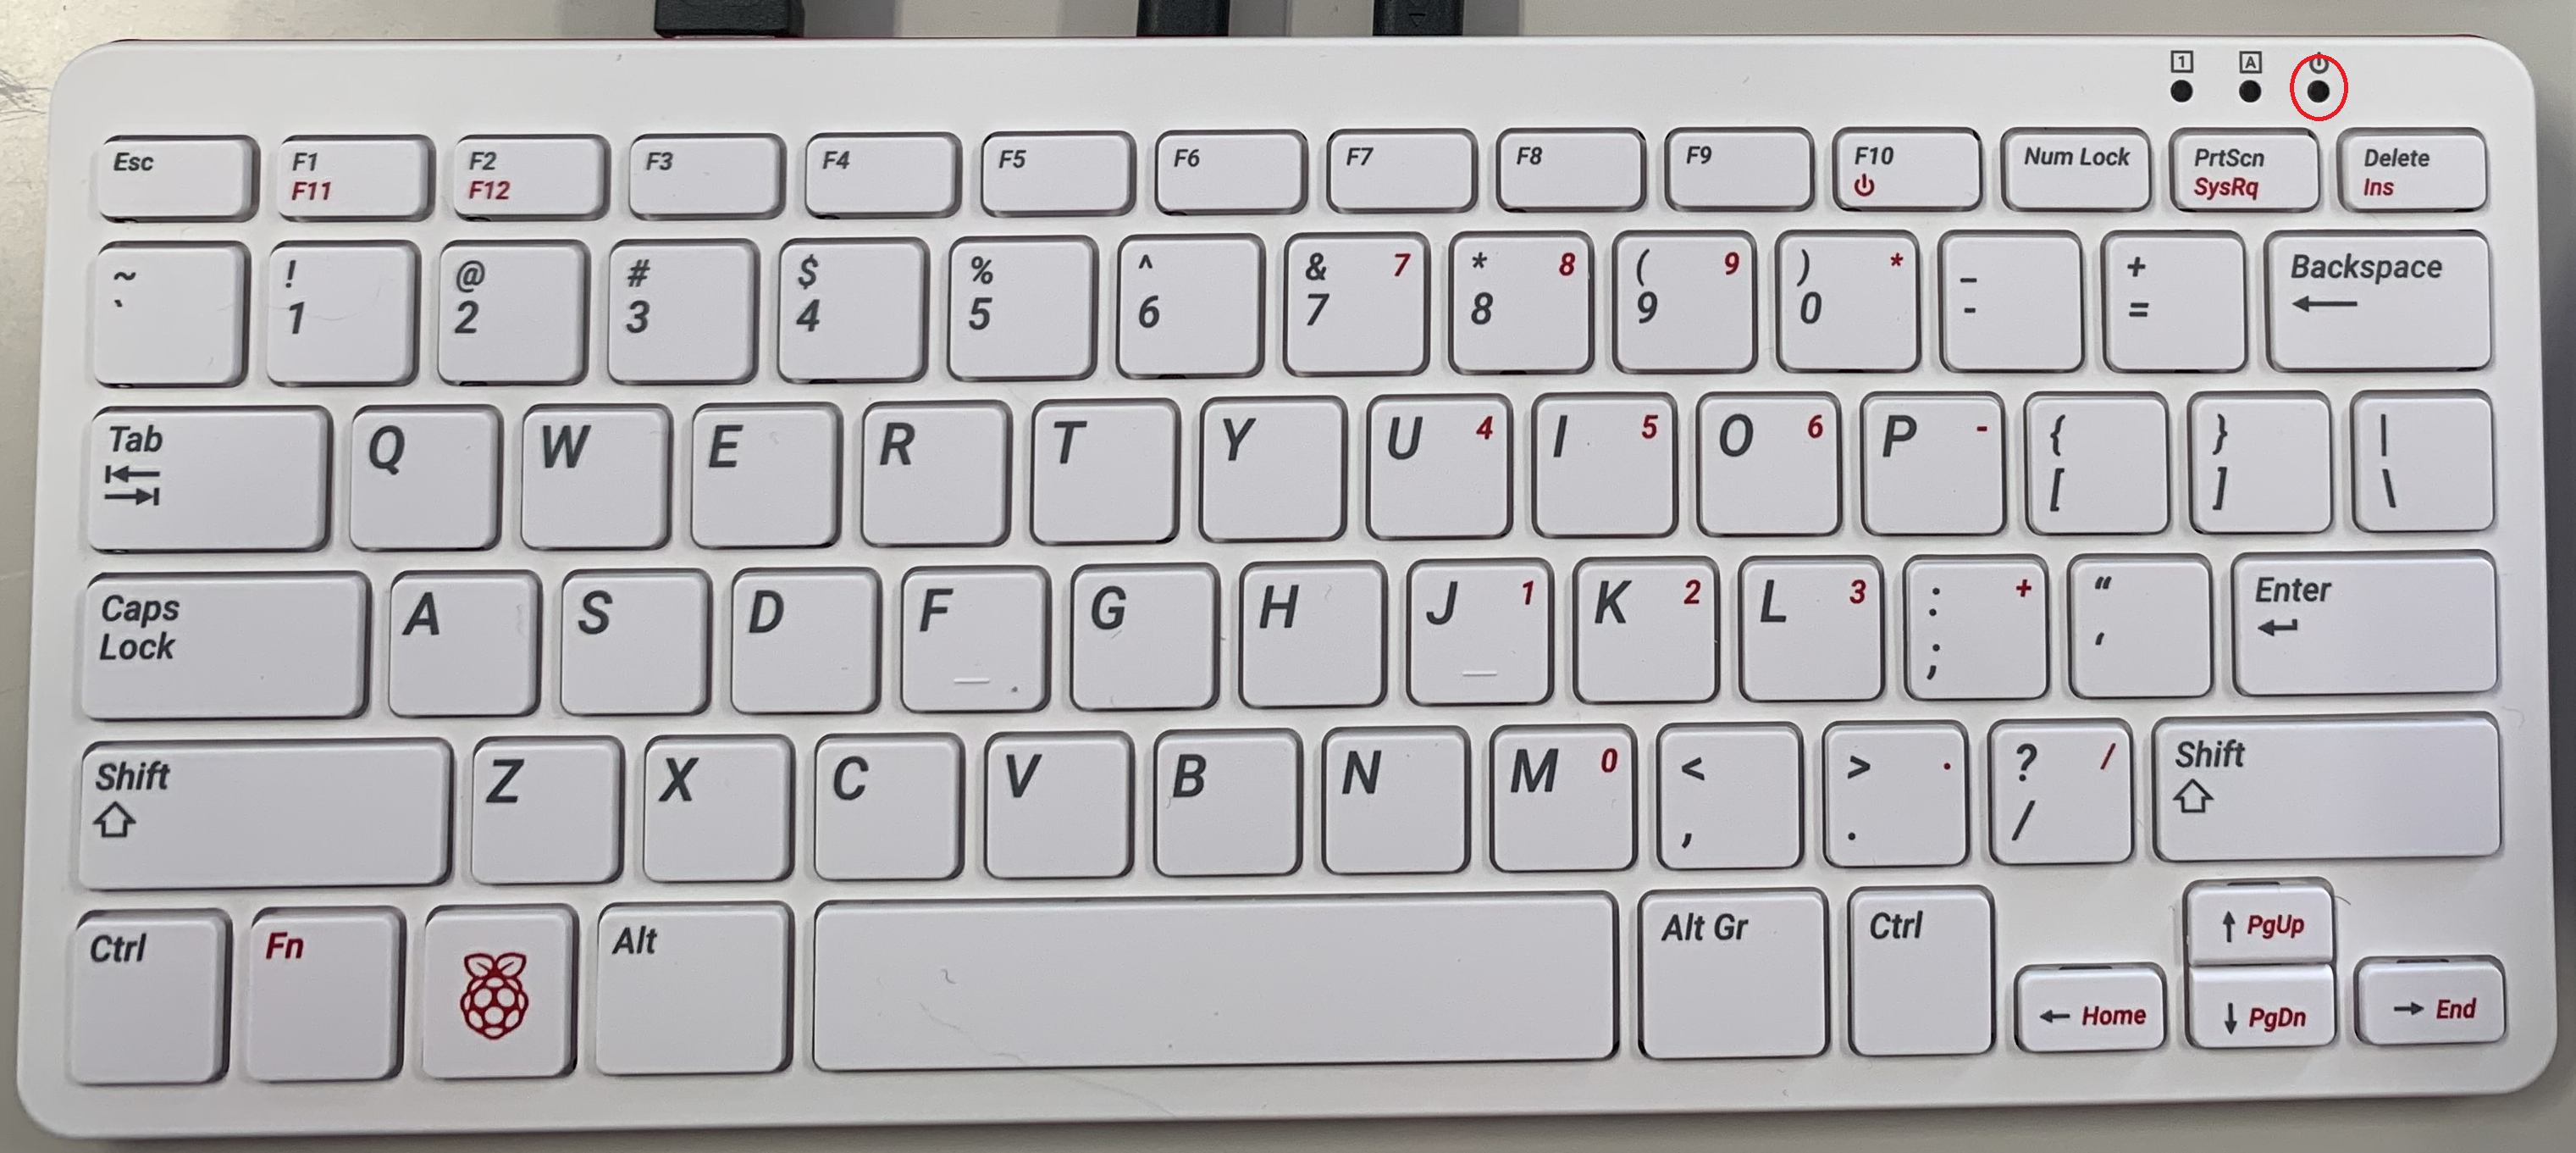
\includegraphics[keepaspectratio, height=35mm]{../../asset/image/textbook-img207x.png}
  \vss}
  \vspace{35mm}
\end{minipage}


%
% subsection 1.4.3
%
\subsection{安全に持ち帰ろう}

ラズベリーパイなどの電子機器はらんぼうに扱うと、簡単に\ruby{壊}{こわ}れてしまいます。
また、静電気にも弱いという\ruby{特徴}{とくちょう}があります。
ラズベリーパイは、必ず\ruby{付属}{ふぞく}の箱に入れて持ち帰りましょう。
この箱は、外からの\ruby{衝撃}{しょうげき}だけでなく、静電気も\ruby{防}{ふせ}いでくれます。
また、microSDカードはなくさないようにラズベリーパイに\ruby{挿}{さ}したままにしておきましょう。


\clearpage

\end{document}
